\chapter{System Requirement Analysis}


\section{System Requirement Analysis}
At system requirement analysis stage the information gathering process is identified a Smart devices fueled by the hyper-connected Internet of Things (IoT) are becoming
ever more prevalent and pervasive in our personal lives. Sensors are everywhere, and the trend will only continue. Today, sensor-equipped industrial equipment is powered by artificial intelligence (AI). Medical devices can self-diagnose and send alerts to patients and doctors to remotely manage healthcare. Automobiles with in-car connectivity can download new features on the fly. Very soon, refrigerators will plan your dinner and ovens will know how to cook it.


%\begin{itemize} 

%\item Generate  the  bill  for  the  user  and  enter  it  in  the  database.
%\item Over the counter charge management.
%\item Preparation of monthly reports.
%\item Status of the parcel.
%\item Built in backup and restore facilities.
%\item hhghfhgh
%\item Trace out the parcel.

%\end{itemize}


\section{Software Process and Development}
The set of general objectives for "Digital India" development were defined by the various \\
% This section type your project contents 
\textbf{Prototype model}\\

The prototyping paradigm begins with requirements gathering. Together with Panning of those aspects of the software that will be visible to the customer/user (e.g. input approaches and output formats).

% This section type your project contents 

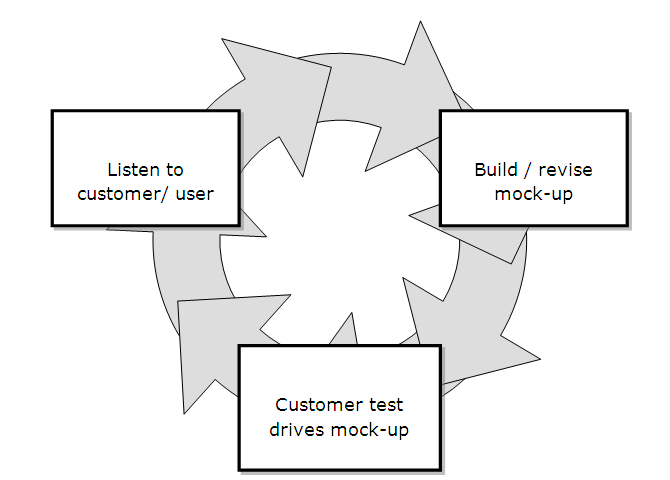
\includegraphics[scale=0.8]{Ch2/prototype.png}

\label{fig:Prototype Model}

% Diagram change as per your project demands

\section{Scope of Proposed System}
Our main purpose is to create a MERN application that helps Customers and other people use their home appliances remotely using their remotely held devices like Mobile phones, tablets, etc.


%\section{Hardware & Software Specifications}


% Write scope of your system.

\section{Technical Specification}
\textbullet \hspace{0.2cm} \textbf{Server}\\
Processor	:	Intel i3\\
RAM          	: 	Min. 512 MB\\
Hard Disk	: 	Min. 512 MB free\\
\textbullet \hspace{0.2cm} \textbf{Client}\\
Processor   	: 	Intel i3 or Above\\
RAM           	: 	Min. 512 MB\\
Hard Disk	: 	Min. 480 MB free\\
\textbullet \hspace{0.2cm} \textbf{Software Specification}\\
Platform	:  	Windows XP\\
Front End	: 	HTML, JavaScript,CSS,React \\
Middle ware	: 	JavaScript,Express,Node\\
Back End	: 	MongoDB \\
Framework: Express\\	
Web Browser: 	Chrome etc. \\


\subsection{Express Framework}
Express is a NodeJS-driven framework, you churning out dynamic, interactive, professional websites in no time.\\

\textbullet \hspace{0.2cm}	It underpins the Model/View/Controller (MVC) approach to web development—a best practice philosophy all developers should adhere to.\\

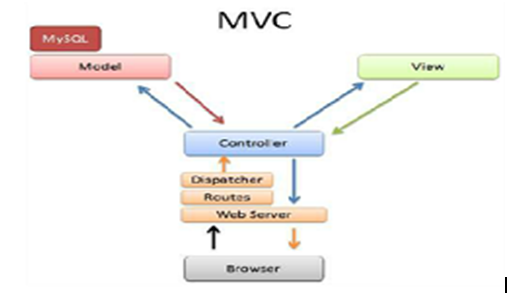
\includegraphics[scale=1.0]{Ch2/mvc.png}


% Diagram change as per your project demands (If required)
\label{fig:MVC Model}

%\textbullet \hspace{0.2cm}It’s built on a linear, easy-to-use folder structure.\\


% This section type your project contents 